%!TeX root = latch_circuit
\documentclass[../main.tex]{subfiles}

\begin{document}
    \section{Latch and overvoltage detection subcircuit}
    The MOSFET driver's inputs are determined from different sources. These sources are positive digital voltage pulses and, thus, a latching subcircuit is needed to maintain a constant digital voltage for driving the MOSFET driver. In this section, the followings are discussed:
    \begin{enumerate}
        \item \nameref{ssec:latch_input_src}
        \item \nameref{ssec:proposed_latch_design}
        \item \nameref{ssec:ovlo_circuit}
    \end{enumerate}

    \pagebreak
    \subsection{Latch subcircuit's input sources and block diagram} \label{ssec:latch_input_src}
    In this project, there are four input sources for the MOSFET driver, and only the first source is for turning on the MOSFET:
    \begin{itemize}
        \item MANUAL\_ON, a momentary switch which the user press to turn on the MOSFET.
        \item ALE, the output from the ALE pin of the INA226 which outputs a positive pulse when the power threshold is exceeded (discussed in latter section).
        \item OVLO (Overvoltage Lockout), the output from a comparator which outputs a HIGH signal if the input supply voltage exceeds a specified threshold (discussed in latter section).
        \item MCU\_CTRL, the output from the MCU.
    \end{itemize}

    \justify
    The following diagram demonstrates the desired latching output, as a result of combining the input sources, for driving the MOSFET driver.

    \begin{figure}[!h]
        \centerline{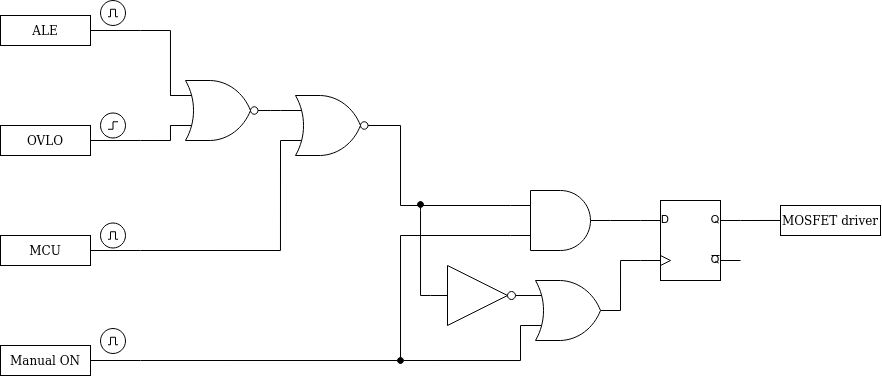
\includegraphics[width=\linewidth]{media/latch_circuit_diagram.png}}
        \caption{Latch subcircuit diagram.}
        \label{fig:latch_circuit_diagram}
    \end{figure} 

    \justify
    The D-latch will only update its held value $Q$ if MANUAL\_ON is HIGH or one of the other source is HIGH. This diagram should not be implemented with discrete logic ICs for the following reasons:
    \begin{itemize}
        \item At least 4 different kind of logic function is needed: \textbf{NOR}, \textbf{AND}, \textbf{OR}, \textbf{D-LATCH}. The \textbf{NOT} function can be constructed from \textbf{NOR} by shorting the inputs of the \textbf{NOR}.
        \item Off-the-shelf logic ICs usually come as: 14-pin package with quad 2-input or triple 3-input gates.
    \end{itemize}

    \justify
    Thus, at least 4 discrete logic ICs is required. With such, many gates are left unused, and the PCB design is clustered and tedious. Instead, a proposed design requiring only 1 op-amp gate is used.

    \pagebreak
    \subsection{Proposed latch subcircuit design} \label{ssec:proposed_latch_design}
    The proposed design is shown in Figure \ref{fig:op_amp_latch_circuit}

    \begin{figure}[!h]
        \centerline{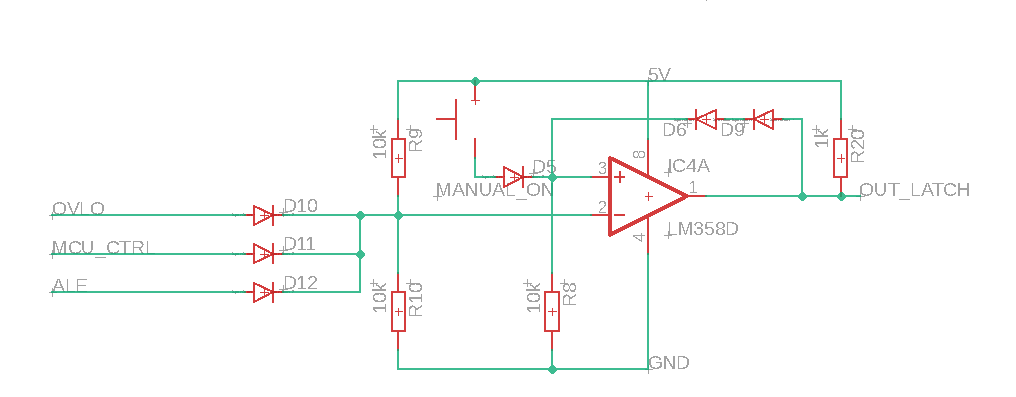
\includegraphics[width=\linewidth]{media/op_amp_latch_circuit.png}}
        \caption{Single op-amp latch subcircuit.}
        \label{fig:op_amp_latch_circuit}
    \end{figure} 

    \begin{itemize}
        \item The resistor $R_9$ and $R_{10}$ create a $2.5V$ potential seen at the inverting input of the op-amp, while the non-inverting input is pull LOW by $R_8$. This setup allows the initial output of the op-amp to be LOW.
        \item The diode $D_6$ and $D_9$ applies a positive feedback to the non-inverting input. With the loop, the non-inverting input will approximate:
        \begin{itemize}
            \item $5V-2\cdot V_{diode\_drop}$ if the output is HIGH.
        \end{itemize}
        \item When the MANUAL\_ON button is pressed, $D_5$ is forward-biased, creating an approximate $4.3V$ at the non-inverting input higher than the $2.5V$ at the invering input. This drives the op-amp's output to be HIGH. Then $D_6$ and $D_9$ is forward biased, latching the non-inverting voltage at $3.6V$, and keeping the op-amp's output HIGH even when the button is released.
        \item The \textbf{NOR} function for the turn-off sources is done by the network of diodes $D_{10}$, $D_{11}$ and $D_{12}$. If any turn-off sources is HIGH, then the non-inverting input's voltage is approximately $4.3V$ higher than the latched voltage at the non-inverting voltage. The op-amp ouptut will be LOW, the non-inverting input is pulled low again. Even when the turn-off sources are no longer HIGH, the inverting input is kept at $2.5V$ created by $R_9$ and $R_{10}$.
    \end{itemize}

    \justify
    With greatly reduced component count, this proposed subcircuit is still able to achieve the desired behaviour established by the diagram in Figure \ref{fig:latch_circuit_diagram}. The op-amp chosen for this subcircuit is the LM393 from Texas Instruments Inc. \cite{LM393}.

    \pagebreak
    \subsection{Overvoltage detection subcircuit} \label{ssec:ovlo_circuit}
    \justify
    The spare op-amp in the LM393 used in latch subcircuit is used to create a simple comparator that outputs HIGH when an overvoltage event is detected. In Figure \ref{fig:ovlo_circuit}, the inverting pin is connected to a LDO regulator AMS1117-1.2V to create a $V_{ref}=1.2V$. $R_{14}$ and $R_{15}$ steps the input supply voltage down by a factor of $1+\dfrac{R_{14}}{R_{15}}= 24.2$, thus, the detection threshold is $1.2V\cdot 24.2=29V$.

    \begin{figure}[!h]
        \centerline{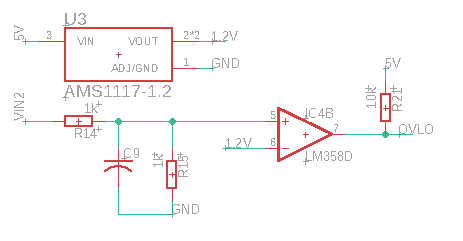
\includegraphics[width=\linewidth]{media/ovlo_circuit.png}}
        \caption{Overvoltage detection subcircuit.}
        \label{fig:ovlo_circuit}
    \end{figure} 
\end{document}